%% LyX 2.0.6 created this file.  For more info, see http://www.lyx.org/.
%% Do not edit unless you really know what you are doing.
\documentclass[11pt,twoside,english,italian]{report}
\renewcommand{\ttdefault}{mathpazo}
\usepackage[T1]{fontenc}
\usepackage[utf8]{inputenc}
\usepackage[a4paper]{geometry}
\geometry{verbose}
\setcounter{secnumdepth}{3}
\setcounter{tocdepth}{3}
\usepackage{fancybox}
\usepackage{calc}
\usepackage{amsmath}
\usepackage{amssymb}
\PassOptionsToPackage{normalem}{ulem}
\usepackage{ulem}

\makeatletter

%%%%%%%%%%%%%%%%%%%%%%%%%%%%%% LyX specific LaTeX commands.
%% Because html converters don't know tabularnewline
\providecommand{\tabularnewline}{\\}

%%%%%%%%%%%%%%%%%%%%%%%%%%%%%% User specified LaTeX commands.

\newlength\tindent
\setlength{\tindent}{\parindent}
\setlength{\parindent}{0pt}
\renewcommand{\indent}{\hspace*{\tindent}}

\title{Logica e Algebra 2}
 
\usepackage{tikz}

\usepackage{color}   %May be necessary if you want to color links
\usepackage{hyperref}
\hypersetup{
    colorlinks=true, %set true if you want colored links
    linktoc=all,     %set to all if you want both sections and subsections linked
    linkcolor=black,  %choose some color if you want links to stand out
}

\usepackage{booktabs}
\usepackage{listings}
\lstset{columns=fullflexible}

\usepackage{wasysym}

\usepackage{amsthm}
\newtheoremstyle{note} % name
{\topsep} 	% Space above
{\topsep} 	% Space below
{\small}		% Body font
{}		% Indent amount
{\small\bfseries}% Theorem head font
{:}		% Punctuation after theorem head
{.5em}	% Space after theorem head
{}		% Theorem head spec (can be left empty, meaning ‘normal’)

\usepackage{fancyhdr}%% Cambia il carattere delle didascalie delle figure %%
\usepackage[font=small,format=plain,labelfont=bf,up,textfont=it,up]{caption}

\usepackage{comment}

%per le tabelle lunghe e particolari
\usepackage{lscape}

\makeatother

\usepackage{babel}
\begin{document}
\tableofcontents{}

\selectlanguage{english}%
\global\long\def\veraw#1#2#3{#1\models_{#2}#3}


\global\long\def\vera#1#2{#1\models#2}


\global\long\def\nonvera#1#2{#1\nvDash#2}


\global\long\def\nonveraw#1#2#3{#1\nvDash_{#2}#3}


\global\long\def\nonSem#1#2{#1\nvdash#2}


\global\long\def\nonTeor#1#2{\nvdash_{#1}#2}


\global\long\def\nonSemW#1#2#3{#1\nvdash_{#2}#3}


\global\long\def\verita#1#2{#1\in V(#2)}


\global\long\def\entail#1#2{#1\models#2}


\global\long\def\semantica#1#2#3{#1\vdash_{#2}#3}


\global\long\def\teolm#1#2{\vdash_{#1}#2}


\global\long\def\semGen#1#2{#1\vdash#2}


\global\long\def\boxx#1{\square#1}


\global\long\def\diam#1{\diamond#1}


\global\long\def\dia{\diamond a}


\global\long\def\boa{\boxx a}


\global\long\def\noa{\neg a}


\global\long\def\forhten#1#2#3{\forall#1#2\implies#3}


\global\long\def\implica#1#2{#1\implies#2}


\global\long\def\teorema#1{\vdash_{\Lambda}#1}


\global\long\def\teorGamma#1{\Gamma\vdash_{\Lambda}#1}


\global\long\def\teoa{\teorGamma a}


\global\long\def\teoremaDi#1{\vdash_{#1}}


\global\long\def\consist{\mbox{\ensuremath{\Lambda}}-consistente}


\global\long\def\consMax{\Lambda-consistente\: massimale}


\global\long\def\veraCanAlfa#1{\vera{M^{\Lambda}}{_{\alpha}}#1}


\global\long\def\veraCA{\vera{M^{\Lambda}}{_{\alpha}}a}


\global\long\def\veraCan#1#2{\vera{M^{\Lambda}}{_{#1}}#2}


\global\long\def\nonveraCan#1#2{\nonveraw{M^{\Lambda}}{#1}{#2}}


\global\long\def\consMaxLog#1{#1-consistente\ massimale}


\global\long\def\relazCAB#1#2{\{a\ |\ \boa\in#1\}\subseteq#2}


\global\long\def\relazCAD#1#2{\{\diamond b\ |\ b\in#2\}\subseteq#1}


\global\long\def\andoria#1{a_{1}\wedge...\wedge a#1}


\global\long\def\andbox#1{\boa_{1}\wedge\dots\wedge\boxx a#1}
\selectlanguage{italian}%




\chapter{Introduzione}

\label{cap:introduction}


\section{Intro}

Se voi signorine finirete questo corso, e se sopravviverete sarete
dispensatori di fbf e pregherete per modellizzare sistemi assurdi
in modo ancora più assurdo, ma fino a quel giorno non siete altro
che buoni annulla convinti che tutti i cretesi sono stupidi e forse
mentono.

Lasciate il formaggio fuori dall'aula.



\chapter{Formule di Logica modale e significato}

$a$ è vera nel mondo $\alpha$, e scriviamo $\mu\models_{\alpha}a$

se 
\begin{itemize}
\item $a$ è una lettera enunciativa allora deve valere $\verita a{\alpha}$ 
\item $a$ è del tipo: $a\lor b$ .... allora.... $\mu\models_{\alpha}a$
oppure $\mu\models_{\alpha}b$ 
\end{itemize}

\section{Relazione seriale}

Ip) Frame F con relazione R seriale

Ts) $\boa\implies\dia$

Dimostrazione:

Se non vale: $\veraw{\mu}{\alpha}{\boa}$ allora immediatemente si
ha la tesi in quanto l'antecedente è falso.

Se invce: $\veraw{\mu}{\alpha}{\boa}$ allora

$\forhten{\beta}{\,:\,\alpha R\beta}{\veraw{\mu}{\beta}a}$ per definizione
di box,

inoltre dato che R seriale per Ip si ha anche che $\exists\beta:\:(\alpha,\beta)\:\in R$

da cui: $\veraw{\mu}{\alpha}{\dia}$ per definizione di diamond (esiste
$\beta$ in relazione con $\alpha$ per la serialità e in $\alpha$
vale $a$ dato che $\veraw{\mu}{\alpha}{\boa}$ )\\


Ip) $\boa\implies\dia$

Ts) Frame F con relazione R seriale

\begin{center}
$ $\begin{center}  
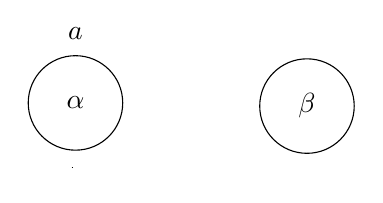
\begin{tikzpicture}[scale=0.2]  
\tikzstyle{every node}+=[inner sep=0pt]  
\draw [black] (24.2,-13) circle (3); 
\draw (24.2,-13) node {$\alpha$};
\draw (24.2,-8.6) node {$\boxx{a}$};
\draw [black] (38.9,-13.2) circle (3);
\draw (38.9,-13.2) node {$\beta$}; 
\draw (24,-17.3) node {\sout{$\dia$}};   
\end{tikzpicture} \end{center}
\par\end{center}

Per assurdo:

Suppongo di trovarmi in un mondo come quello in figura (wow) in cui
\mbox{$\veraw{\mu}{\alpha}{\boa}$ }, e suppongo che la relazione
R del frame NON sia seriale cioè $\sim\exists\beta:(\alpha R\beta)$,
se è così vale sicuramente $\veraw{\mu}a{\boa}$ (dato che $\alpha$
non ha successori) , d'altra parte per come è il mondo considerato,
cioè si nega la tesi, assurdo\sout{.}


\section{Relazione riflessiva}

Ip) R riflessiva

Ts) $\boa\implies a$

se l'antecedente è falso il teorema è dimostrato, consideriamo il
caso in cui l'antecedente è vero:

$\veraw{\mu}{\alpha}{\boa}$

poichè il frame è riflessivo, abbiamo $\alpha R\alpha$, e quindi
varrà:

$\veraw{\mu}{\alpha}a$

e la tesi è dimostrata.

\begin{center} 
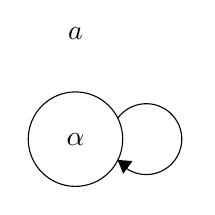
\begin{tikzpicture}[scale=0.2] 
\tikzstyle{every node}+=[inner sep=0pt] 
\draw [black] (32.4,-24.8) circle (3); 
\draw (32.4,-24.8) node {$\alpha$}; 
\draw (32.4,-20.6) node {$\boa$}; 
\draw (32.4,-18.1) node {$a$}; 
\draw [black] (35.08,-23.477) arc (144:-144:2.25); 
\fill [black] (35.08,-26.12) -- (35.43,-27) -- (36.02,-26.19); 
\end{tikzpicture} \end{center}

Ip) $\boa\implies a$

Ts) R è riflessiva

Supponiamo per assurdo che R non sia riflessiva, allora prendiamo
uno stato $\alpha$ tale che $\nexists\beta:\,\alpha R\beta$. Allora
si avrà che:

$\veraw{\mu}{\alpha}{\boa}\wedge\nonveraw{\mu}{\alpha}a$

che è assurdo perchè contraddice la tesi. La tesi allora è valida.

\begin{center} 
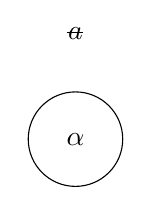
\begin{tikzpicture}[scale=0.2] 
\tikzstyle{every node}+=[inner sep=0pt] 
\draw [black] (32.4,-24.8) circle (3); 
\draw (32.4,-24.8) node {$\alpha$}; 
\draw (32.4,-20.6) node {$\boa$}; 
\draw (32.4,-18.1) node {\sout{$a$}}; 
\end{tikzpicture} 
\end{center}


\section{Relazione simmetrica}

Ip) R simmetrica

Ts) $a\implies\boxx{\dia}$

Suppongo che $\veraw{\mu}{\alpha}a$ (se no avrei già la tesi), due
casi:

\textbf{Caso 1}: Da $\alpha$ non parte nessun arco, allora sicuramente
$\veraw{\mu}{\alpha}{\boxx x}$ con $x$ qualsiasi e in particolare
$\veraw{\mu}{\alpha}{\boxx{\dia}}$

\begin{center}
\begin{center} 
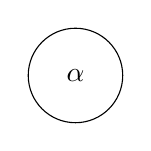
\begin{tikzpicture}[scale=0.2] 
\tikzstyle{every node}+=[inner sep=0pt] 
\draw [black] (24.2,-13) circle (3);
\draw (24.2,-13) node {$\alpha$};
\end{tikzpicture}
\end{center} 
\par\end{center}

\textbf{Caso 2}: Esiste almeno un $\beta$ tale che $\alpha R\beta$.

\begin{center}
\begin{center} 
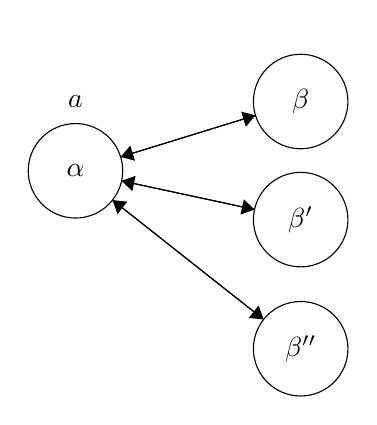
\begin{tikzpicture}[scale=0.2] 
\tikzstyle{every node}+=[inner sep=0pt] 
\draw [black] (24.2,-12.7) circle (3); 
\draw (24.2,-12.7) node {$\alpha$};
\draw (24.2,-8.3) node {$a$};  
\draw [black] (38.5,-8.3) circle (3);
 \draw (38.5,-8.3) node {$\beta$}; 
\draw [black] (38.5,-15.8) circle (3);  
\draw (38.5,-15.8) node {$\beta'$};  
\draw [black] (38.5,-24) circle (3);  
\draw (38.5,-24) node {$\beta''$}; 
\draw (38.5,-3.7) node {$\dia$};
\draw (38.5,-11.7) node {$\dia$};  \draw (38.5,-20.2) node {$\dia$}; 
\draw [black] (27.07,-11.82) -- (35.63,-9.18); \fill [black] (35.63,-9.18) -- (34.72,-8.94) -- (35.02,-9.9);  \draw [black] (35.63,-9.18) -- (27.07,-11.82);  \fill [black] (27.07,-11.82) -- (27.98,-12.06) -- (27.68,-11.1); \draw [black] (27.13,-13.34) -- (35.57,-15.16); \fill [black] (35.57,-15.16) -- (34.89,-14.51) -- (34.68,-15.48); \draw [black] (35.57,-15.16) -- (27.13,-13.34);  \fill [black] (27.13,-13.34) -- (27.81,-13.99) -- (28.02,-13.02);  \draw [black] (26.55,-14.56) -- (36.15,-22.14); \fill [black] (36.15,-22.14) -- (35.83,-21.25) -- (35.21,-22.04);  \draw [black] (36.15,-22.14) -- (26.55,-14.56);  \fill [black] (26.55,-14.56) -- (26.87,-15.45) -- (27.49,-14.66); \end{tikzpicture} \end{center}
\par\end{center}

Dato che la relazione è simmetrica se $\alpha R\beta$ allora \textbf{$\beta R\alpha$.}
Dato che $\veraw{\mu}{\alpha}a,$ in ognuno di questi $\beta$, $\beta'$,$\beta''$
ecc. vale $\dia$ perché ognuno di loro è in relazione con $\alpha$.

Allora per ognuno di questi $\beta$ si ha $\veraw{\mu}{\beta}{\dia}$,
(esiste infatti un mondo, $\alpha$, in cui vale $a$) da cui: $\veraw{\mu}{\alpha}{\boxx{\dia}}$
\\


Ip) $a\implies\boxx{\dia}$

Ts) R simmetrica

Per assurdo:

suppongo R non sia simmetrica e considero un frame con soli $\alpha$
e $\beta$ e in cui $R=\{(\alpha,\beta)\}$ . In questo frame considero
un modello con funzione di verità tale che: $V(A)=\{\alpha\}$.

In $\beta$ non vale $\dia$ perché $\beta$ non è in relazione con
nessun mondo, per questo: $\nonveraw{\mu}{\alpha}{\boxx{\dia}}$

\begin{center}
\begin{center}  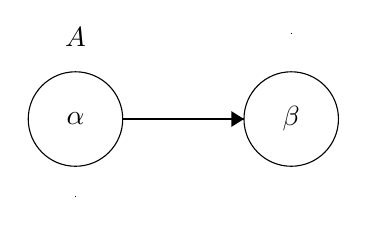
\begin{tikzpicture}[scale=0.2] \tikzstyle{every node}+=[inner sep=0pt]  \draw [black] (24.2,-12.7) circle (3);  \draw (24.2,-12.7) node {$\alpha$}; 
\draw (24.2,-7.5) node {$A$};
\draw [black] (37.9,-12.7) circle (3); \draw (37.9,-12.7) node {$\beta$};
\draw (37.9,-7.5) node {\sout{$\dia$}}; 
\draw (24.2,-17.8) node {\sout{$\boxx{\dia}$}}; 
\draw [black] (27.2,-12.7) -- (34.9,-12.7); \fill [black] (34.9,-12.7) -- (34.1,-12.2) -- (34.1,-13.2);  \end{tikzpicture} \end{center}
\par\end{center}

$ $


\section{Relazione Transitiva}

Ip) R relazione transitiva

Ts) $\boa\implies\boxx{\boa}$

Se $\nonveraw{\mu}{\alpha}{\boa}$ la tesi è dimostrata, consideriamo
allora il caso in cui $\veraw{\mu}{\alpha}{\boa}$

per ipotesi:

$\exists\beta\,:\,(\alpha,\beta)\,\in R\,(\beta,\gamma)\,\in R$

allora abbiamo che:

$(\alpha,\gamma)\,\in R$

$\veraw{\mu}{\gamma}a$ 

e quindi varrà ovviamente che:

$\veraw{\mu}{\beta}a$

da cui segue:

$\veraw{\mu}{\alpha}{\boxx{\boa}}$ 

e la tesi è dimostrata.

\begin{center} \begin{tikzpicture}[scale=0.2] 
\tikzstyle{every node}+=[inner sep=0pt] 
\draw [black] (16,-26.5) circle (3); 
\draw (16,-26.5) node {$\alpha$}; 
\draw [black] (36.8,-16.1) circle (3); 
\draw (36.8,-16.1) node {$\beta_1$}; 
\draw [black] (54.2,-25.4) circle (3); 
\draw (54.2,-25.4) node {$\gamma$}; 
\draw [black] (37.5,-38.1) circle (3); 
\draw (37.5,-38.1) node {$\beta_2$}; 
\draw (15.9,-21.5) node {$\boa$}; 
\draw (37.5,-33.4) node {$\boa$}; 
\draw (15.9,-18) node {$\boxx{\boa}$}; 
\draw (36.8,-11.9) node {$\boa$}; 
\draw (53.6,-20.6) node {$a$}; 
\draw [black] (18.68,-25.16) -- (34.12,-17.44); 
\fill [black] (34.12,-17.44) -- (33.18,-17.35) -- (33.62,-18.25); 
\draw [black] (39.45,-17.51) -- (51.55,-23.99); \fill [black] (51.55,-23.99) -- (51.08,-23.17) -- (50.61,-24.05); 
\draw [black] (19,-26.41) -- (51.2,-25.49); \fill [black] (51.2,-25.49) -- (50.39,-25.01) -- (50.42,-26.01); 
\draw [black] (18.64,-27.92) -- (34.86,-36.68); 
\fill [black] (34.86,-36.68) -- (34.39,-35.86) -- (33.92,-36.74); 
\end{tikzpicture} 
\end{center}

Ip) $\boa\implies\boxx{\boa}$

Ts) R relazione transitiva

supponiamo per assurdo che esista uno stato$\alpha$ per cui non vale
la proprietà transitiva

consideriamo il caso in cui valga la seguente funzione di valutazione:

$V(a)=\{S\,|\,(\alpha,\delta)\,\in R\}$ 

Allora a sarà vera in $\beta$, ma non in $\gamma$. per cui in $\alpha$
sarà vera $\boa$ ma non $\boxx{\boa}$

\begin{center} 
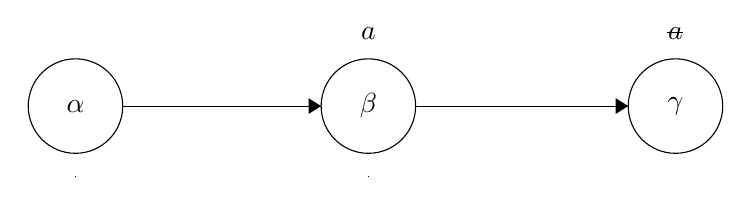
\begin{tikzpicture}[scale=0.2] \tikzstyle{every node}+=[inner sep=0pt] 
\draw [black] (16,-28.2) circle (3); 
\draw (16,-28.2) node {$\alpha$}; 
\draw [black] (34.6,-28.2) circle (3); 
\draw (34.6,-28.2) node {$\beta$}; 
\draw [black] (54.1,-28.2) circle (3); 
\draw (54.1,-28.2) node {$\gamma$}; 
\draw (16,-23.6) node {$\boa$}; 
\draw (34.6,-23.6) node {$a$}; 
\draw (54.1,-23.6) node {\sout{$a$}}; 
\draw (16,-32.9) node {\sout{$\boxx{\boa}$}}; 
\draw (34.6,-32.9) node {\sout{$\boa$}}; 
\draw [black] (19,-28.2) -- (31.6,-28.2); 
\fill [black] (31.6,-28.2) -- (30.8,-27.7) -- (30.8,-28.7); 
\draw [black] (37.6,-28.2) -- (51.1,-28.2); 
\fill [black] (51.1,-28.2) -- (50.3,-27.7) -- (50.3,-28.7); 
\end{tikzpicture} 
\end{center}




\section{Funzione parziale}

\begin{tabular}{|c|c|c|}
\hline 
$\diam a\implies\boxx a$  & funzione parziale  & $\forhten{\alpha}{:\,\alpha R\beta,\:\beta R\gamma}{\beta}=\gamma$\tabularnewline
\hline 
\end{tabular}

Funzione parziale, dimostrazione\\


Ip) funzione parziale

Ts) $\diam a\implies\boxx a$ 

$\diam{}a$ falsa allora dato che l'antecedente è falso di ha $\implica{\diam{}a}{\boxx a}$

$\diam{}a$ vera allora $\exists\beta$:$\alpha R\beta$ e$\in V(\beta)$,
ma dato che la funzione è parziale questo $\beta$ è unico !

da cui $\vera{\mu}{\implica{\diamond a}{\boxx a}}$

Ip) $\diam a\implies\boxx a$ 

Ts) funzione parziale

Per assurdo: suppongo non che la funzione non sia parziale. Se è così
$\exists\alpha:$ $\alpha R\beta,$ $\alpha R\gamma$, considero un
modello in cui V(A) = \{$\beta$ \} , $\boxx A$ non vale in $\alpha$
dato che A è falsa in $\gamma$, il che contraddice l'ipotesi (BAM!)\\
 \\
 


\section{Funzione totale}

\begin{tabular}{|c|c|c|}
\hline 
$\dia\iff\boxx a$  & funzione totale  & $\forall\alpha\exists\,!\,\beta:\:\alpha R\beta$ \tabularnewline
\hline 
\end{tabular}\\
 \\


non ci sono ``conti'' da fare, R è seriale sse R è seriale $\boxx a\implies\diam a$
, e se R è una funzione parziale $\implica{\diam a}{\boxx a}$

quindi dato che l'implica prevede un and di implica da una parte e
dall'altra per definizione abbiamo la tesi

.


\section{Relazione euclidea}

\begin{tabular}{|c|c|c|}
\hline 
$\dia\implies\boxx{\diam a}$  & relazione euclidea  & $\forhten{\alpha,\beta,\gamma}{:\:(\alpha R\beta,\:\alpha R\gamma)}{\beta}R\gamma$
da cui anche: $\beta$R$\beta$, $\gamma R\gamma$, $\gamma$R$\beta$\tabularnewline
\hline 
\end{tabular}\\
 \\


Ip) relazione euclidea

Ts) $\diam a\implies\boxx{\diam a}$

Suppongo sia vero l'antecedente (se falso ho finito), quindi vale:
$\dia$ da cui: $\vera{\mu}{\dia}$

dato che $\dia$ si ha che esiste almeno un $\beta$ tale che in beta
vale a

solo un beta: autoanello perché euclidea e quindi $\boxx{\dia}$

diversi beta: ognuno dei vari $\beta'$, $\beta''$ , ecc. sono in
relazione con $\beta$, dato che la relazione è euclidea, pertanto
dato che in $\beta$ vale $a$, in ognuno di loro vale $\dia$ \\


\begin{center}
 \begin{center}  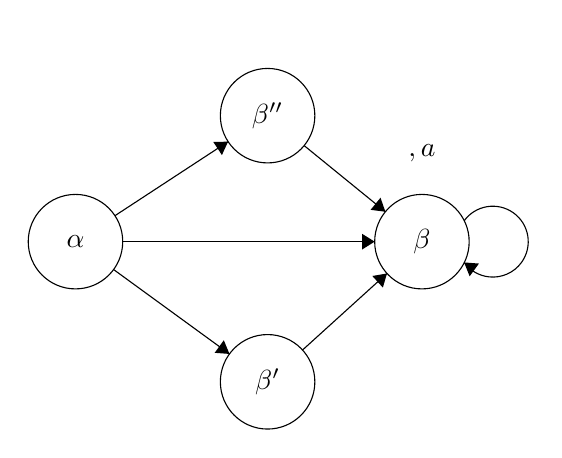
\begin{tikzpicture}[scale=0.2]  \tikzstyle{every node}+=[inner sep=0pt] \draw [black] (24.5,-18.4) circle (3); \draw (24.5,-18.4) node {$\alpha$}; \draw [black] (46.5,-18.4) circle (3);  \draw (46.5,-18.4) node {$\beta$}; \draw [black] (36.7,-27.3) circle (3);  \draw (36.7,-27.3) node {$\beta'$}; \draw (23.9,-12.8) node {$\dia$}; \draw (46.5,-12.8) node {$\dia, a$}; \draw (36.7,-22.1) node {$\dia$}; \draw [black] (36.7,-10.4) circle (3); \draw (36.7,-10.4) node {$\beta''$}; \draw (36.7,-4.9) node {$\dia$}; \draw [black] (27.5,-18.4) -- (43.5,-18.4);  \fill [black] (43.5,-18.4) -- (42.7,-17.9) -- (42.7,-18.9); \draw [black] (26.92,-20.17) -- (34.28,-25.53);  \fill [black] (34.28,-25.53) -- (33.92,-24.66) -- (33.34,-25.46);  \draw [black] (27.01,-16.75) -- (34.19,-12.05);  \fill [black] (34.19,-12.05) -- (33.25,-12.07) -- (33.8,-12.9);  \draw [black] (49.18,-17.077) arc (144:-144:2.25); \fill [black] (49.18,-19.72) -- (49.53,-20.6) -- (50.12,-19.79); \draw [black] (39.02,-12.3) -- (44.18,-16.5); \fill [black] (44.18,-16.5) -- (43.87,-15.61) -- (43.24,-16.38); \draw [black] (38.92,-25.28) -- (44.28,-20.42); \fill [black] (44.28,-20.42) -- (43.35,-20.58) -- (44.02,-21.32);  \end{tikzpicture} \end{center} 
\par\end{center}

Ip)$\dia\implies\boxx{\diam a}$

Ts) relazione euclidea

Per assurdo, suppondo valga ip) ma non la tesi

Considero un Frame in cui: $\alpha R\beta,$ $\alpha R\gamma,$ $\beta R\gamma$
ma NON $\beta R\gamma$ cioè si ha un frammento in cui non vale l'euclidea.
Poniamo che il modello sia tale che $V(A)$$=\{\gamma\}$

In queste ipotesi vale $\dia$ dato che in $\gamma$ vale $a$. In
$\beta$ non vale $a$ e neppure $\dia$ perché non ha ``uscite'',
da cui in $a$ non vale $\boxx{\dia}$ contraddicendo così l'ipotesi
(BAM!) 


\section{Relazione Debolmente Densa}

\begin{tabular}{|c|c|c|}
\hline 
$\dia\implies\diam{\diam a}$  & relazione debolmente densa  & $\forhten{\alpha,\beta}{:\:(\alpha R\beta)}{\exists\gamma:\,(\alpha R\gamma\wedge\gamma R\beta)}$\tabularnewline
\hline 
\end{tabular}

Ip) R debolmente densa

Ts) $\dia\implies\diam{\diam a}$ 

supponiamo che sia vero l'antecedente (se è falso la tesi è dimostrata)
avremo quindi:

$\veraw{\mu}{\alpha}{\dia}$

allora segue che:

$\exists\beta:\,\veraw{\mu}{\beta}a$

ma poichè la relazione è debolmente densa, si avrà che:

$\exists\gamma:\,(\alpha R\gamma\wedge\gamma R\beta)$

poichè in $\beta$ è vera a, allora segue:

$\veraw{\mu}{\gamma}{\dia}$

da cui segue:

$\veraw{\mu}{\alpha}{\diam{\dia}}$

e la tesi è dimostrata.

\begin{center} 
\begin{tikzpicture}[scale=0.2] 
\tikzstyle{every node}+=[inner sep=0pt] 
\draw [black] (18.2,-20) circle (3); 
\draw (18.2,-20) node {$\alpha$}; 
\draw [black] (47.3,-20) circle (3); 
\draw (47.3,-20) node {$\beta$}; 
\draw [black] (33.6,-32.3) circle (3); 
\draw (33.6,-32.3) node {$\gamma$}; 
\draw (18.2,-15.1) node {$\dia$}; 
\draw (18.2,-12.4) node {$\diam{\dia}$}; 
\draw (47.3,-15.1) node {$a$}; 
\draw (33.6,-36.9) node {$\dia$}; 
\draw [black] (21.2,-20) -- (44.3,-20); 
\fill [black] (44.3,-20) -- (43.5,-19.5) -- (43.5,-20.5); 
\draw [black] (20.54,-21.87) -- (31.26,-30.43); 
\fill [black] (31.26,-30.43) -- (30.94,-29.54) -- (30.32,-30.32); 
\draw [black] (35.83,-30.3) -- (45.07,-22); 
\fill [black] (45.07,-22) -- (44.14,-22.17) -- (44.81,-22.91); 
\end{tikzpicture} 
\end{center} 

Ip) $\dia\implies\diam{\diam a}$ 

Ts) R debolmente densa

Supponiamo per assurdo che R non sia debolmente densa.

Supponiamo allora che esista uno stato $\beta$ pozzo e $\alpha R\beta$
in cui sia vera a

segue che:

$\veraw{\mu}{\alpha}{\dia}$

ma avremo anche che:

$\nonveraw{\mu}{\beta}{\dia}$

e allora otteniamo:

$\nonveraw{\mu}{\alpha}{\diam{\dia}}$

che è assurdo perchè contraddice l'ipotesi, e quindi la tesi è dimostrata.

\begin{center} 
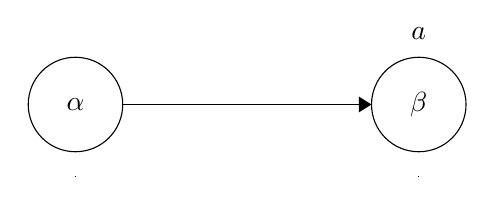
\begin{tikzpicture}[scale=0.2] 
\tikzstyle{every node}+=[inner sep=0pt] 
\draw [black] (22,-22.3) circle (3); 
\draw (22,-22.3) node {$\alpha$}; 
\draw [black] (43.8,-22.3) circle (3); 
\draw (43.8,-22.3) node {$\beta$}; 
\draw (22,-17.8) node {$\dia$}; 
\draw (43.8,-17.8) node {$a$}; 
\draw (43.8,-27.1) node {\sout{$\dia$}}; 
\draw (22,-27.1) node {\sout{$\diam{\dia}$}}; 
\draw [black] (25,-22.3) -- (40.8,-22.3); 
\fill [black] (40.8,-22.3) -- (40,-21.8) -- (40,-22.8); 
\end{tikzpicture} 
\end{center}


\section{Relazione Diretta}

\begin{tabular}{|c|c|c|}
\hline 
$\diam{\boa}\implies\boxx{\dia}$  & relazione diretta  & $\forhten{\alpha,\beta}{,\gamma:\:(\alpha R\beta\wedge\alpha R\gamma)}{\exists\delta:\,(\beta R\delta\wedge\gamma R\delta)}$\tabularnewline
\hline 
\end{tabular}

Ip) R è diretta

Ts) $\diam{\boa}\implies\boxx{\dia}$ 

Se l'antecedente è falso, il teorema è dimostrato. poniamoci quindi
nel caso:

$\veraw{\mu}{\alpha}{\diam{\boa}}$

avremo allora che:

$\exists\beta:\,\alpha R\beta\wedge\veraw{\mu}{\beta}{\boa}$

allora necessariamente si avrà che:

$\exists\delta:\,\beta R\delta\wedge\veraw{\mu}{\delta}a$

allora si avrà che:

$\veraw{\mu}{\beta}{\dia}$

prendiamo ora un qualsiasi mondo$\gamma$ tale che $\alpha R\gamma$,
poichè la relazione è diretta si avrà $\gamma R\delta$, e quindi:

$\veraw{\mu}{\gamma}{\dia}$

e allora possiamo osservare che vale:

$\veraw{\mu}{\alpha}{\boxx{\dia}}$

e la tesi è dimostrata

\begin{center} 
\begin{tikzpicture}[scale=0.2] 
\tikzstyle{every node}+=[inner sep=0pt] 
\draw [black] (17.1,-28) circle (3); 
\draw (17.1,-28) node {$\alpha$}; 
\draw [black] (33.1,-19.2) circle (3); 
\draw (33.1,-19.2) node {$\beta$}; 
\draw [black] (33.1,-38.3) circle (3); 
\draw (33.1,-38.3) node {$\gamma$}; 
\draw [black] (48,-28) circle (3); 
\draw (48,-28) node {$\delta$}; 
\draw (17.1,-23.7) node {$\diam{\boa}$}; 
\draw (33.1,-14.3) node {$\boa$}; 
\draw (48,-23.1) node {$a$}; 
\draw (33.1,-42.8) node {$\dia$}; 
\draw (17.1,-21.1) node {$\boxx{\dia}$}; 
\draw (33.1,-11.7) node {$\dia$}; 
\draw [black] (19.62,-29.62) -- (30.58,-36.68); 
\fill [black] (30.58,-36.68) -- (30.18,-35.82) -- (29.63,-36.66); 
\draw [black] (19.73,-26.55) -- (30.47,-20.65); 
\fill [black] (30.47,-20.65) -- (29.53,-20.59) -- (30.01,-21.47); 
\draw [black] (35.68,-20.73) -- (45.42,-26.47); 
\fill [black] (45.42,-26.47) -- (44.98,-25.64) -- (44.47,-26.5); 
\draw [black] (35.57,-36.59) -- (45.53,-29.71); 
\fill [black] (45.53,-29.71) -- (44.59,-29.75) -- (45.16,-30.57); 
\end{tikzpicture} 
\end{center}

Ip) $\diam{\boa}\implies\boxx{\dia}$ 

Ts) R è diretta

Supponiamo per assurdo R non diretta.

Consideriamo la funzione di valutazione:

$V(a)=\{\delta|\beta R\delta\}$

supponiamo che:

$\exists\alpha:\,\veraw{\alpha R\beta\wedge\mu}{\alpha}{\diam{\boa}}$

allora si avrà:

$\veraw{\mu}{\beta}{\boa}$

Prendiamo ora un qualsiasi mondo $\gamma$ tale che $\alpha R\gamma$,
e supponiamo che:

$\nexists\eta:\,\gamma R\eta$

Si avrà dunque che

$\nonveraw{\mu}{\gamma}{\dia}$

allora avremo che:

$\nonveraw{\mu}{\alpha}{\boxx{\dia}}$

che è assurdo, perchè contraddice la tesi. La tesi è allora valida.

\begin{center} 
\begin{tikzpicture}[scale=0.2] \tikzstyle{every node}+=[inner sep=0pt] 
\draw [black] (16.5,-26) circle (3); 
\draw (16.5,-26) node {$\alpha$}; 
\draw [black] (32.1,-15.3) circle (3); 
\draw (32.1,-15.3) node {$\beta$}; 
\draw [black] (46.9,-26) circle (3); 
\draw (46.9,-26) node {$\delta$}; 
\draw [black] (32.1,-37.6) circle (3); 
\draw (32.1,-37.6) node {$\gamma$}; 
\draw (16.5,-21.3) node {$\diam{\boa}$}; 
\draw (31.9,-10.5) node {$\boa$}; 
\draw (46.9,-21.3) node {$a$}; 
\draw (31.9,-32.8) node {\sout{$\dia$}}; 
\draw (16.5,-18.9) node {\sout{$\boxx{\dia}$}}; 
\draw [black] (18.97,-24.3) -- (29.63,-17); 
\fill [black] (29.63,-17) -- (28.68,-17.04) -- (29.25,-17.86); 
\draw [black] (34.53,-17.06) -- (44.47,-24.24); 
\fill [black] (44.47,-24.24) -- (44.11,-23.37) -- (43.53,-24.18); 
\draw [black] (18.91,-27.79) -- (29.69,-35.81); 
\fill [black] (29.69,-35.81) -- (29.35,-34.93) -- (28.75,-35.73); 
\end{tikzpicture} 
\end{center}


\section{Relazione Debolmente Connessa}

\begin{tabular}{|c|c|c|}
\hline 
$\boxx{(a\wedge\boa\implies b)}\vee\boxx{(b\wedge\boxx b\implies a)}$  & relazione debolmente connessa  & $\forhten{\alpha,\beta}{:\:(\alpha R\beta\wedge\alpha R\gamma)}{(\beta R\gamma\vee\beta=\gamma\vee\gamma R\beta)}$\tabularnewline
\hline 
\end{tabular}

Ip) R debolmente connessa

Ts) $\boxx{(a\wedge\boa\implies b)}\vee\boxx{(b\wedge\boxx b\implies a)}$

Se il primo termine è vero, il teorema è verificato. allora supponiamo
che:

$\nonveraw{\mu}{\alpha}{\boxx{(a\wedge\boa\implies b)}}$

ne consegue che:

$\nonveraw{\mu}{\beta}{a\wedge\boa\implies b}$

che si ha solo se valgono:

$\nonveraw{\mu}{\beta}b$

$\veraw{\mu}{\beta}{a\wedge\boa}$

Dobbiamo allora verificare 3 casi:

\textbf{Caso 1 }

se da $\alpha$ non esco in altri stati, poichè è falsa b, allora:

$\veraw{\mu}{\beta}{b\wedge\boxx b\implies a}$

da cui segue che:

$\veraw{\mu}{\alpha}{\boxx{(b\wedge\boxx b\implies a)}}$

E la tesi è verificata.

\begin{center} 
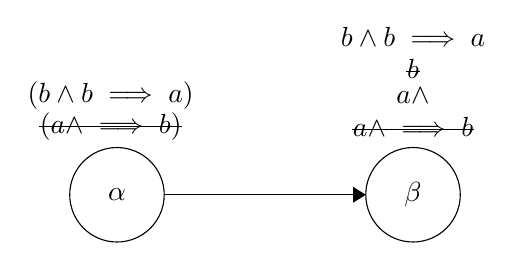
\begin{tikzpicture}[scale=0.2] 
\tikzstyle{every node}+=[inner sep=0pt] 
\draw [black] (21.9,-20.5) circle (3); 
\draw (21.9,-20.5) node {$\alpha$}; 
\draw [black] (40.7,-20.5) circle (3); 
\draw (40.7,-20.5) node {$\beta$}; 
\draw (21.5,-16.2) node {\sout{$\boxx{(a\wedge\boa\implies b)}$}}; 
\draw (21.5,-14.2) node {$\boxx{(b\wedge\boxx b\implies a)}$}; 
\draw (40.7,-16.2) node {\sout{$a\wedge\boa\implies b$}}; 
\draw (40.7,-14.2) node {$a\wedge\boa$}; 
\draw (40.7,-12.5) node {\sout{$b$}}; 
\draw (40.7,-10.5) node {$b\wedge\boxx b\implies a$}; 
\draw [black] (24.9,-20.5) -- (37.7,-20.5); 
\fill [black] (37.7,-20.5) -- (36.9,-20) -- (36.9,-21); 
\end{tikzpicture} 
\end{center}

\textbf{Caso 2 }

Se da $\alpha$ vado in un altro mondo $\gamma$ raggiungibile da
$\beta$:

$\veraw{\mu}{\gamma}a$

e quindi:

$\veraw{\mu}{\beta}{b\wedge\boxx b\implies a}$

da cui segue che:

$\veraw{\mu}{\alpha}{\boxx{(b\wedge\boxx b\implies a)}}$

E la tesi è verificata.

\begin{center} 
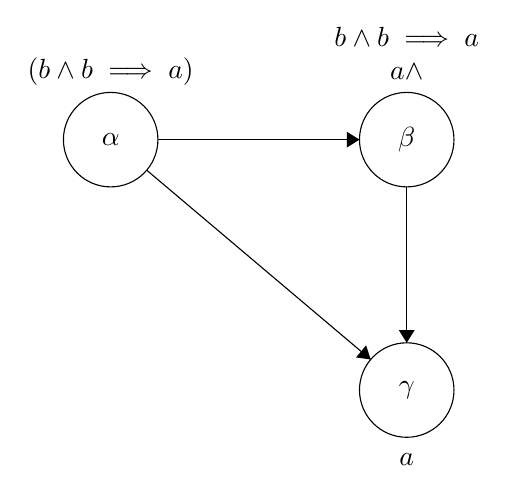
\begin{tikzpicture}[scale=0.2] 
\tikzstyle{every node}+=[inner sep=0pt] 
\draw [black] (21.9,-20.5) circle (3); 
\draw (21.9,-20.5) node {$\alpha$}; 
\draw [black] (40.7,-20.5) circle (3); 
\draw (40.7,-20.5) node {$\beta$}; 
\draw [black] (40.7,-36.4) circle (3); 
\draw (40.7,-36.4) node {$\gamma$}; 
\draw (40.7,-16.2) node {$a\wedge\boa$}; 
\draw (40.7,-40.8) node {$a$}; 
\draw (40.7,-14) node {$b\wedge\boxx{b}\implies a$}; 
\draw (21.9,-16.2) node {$\boxx{(b\wedge\boxx{b}\implies a)}$}; 
\draw [black] (24.9,-20.5) -- (37.7,-20.5); 
\fill [black] (37.7,-20.5) -- (36.9,-20) -- (36.9,-21); 
\draw [black] (40.7,-23.5) -- (40.7,-33.4); 
\fill [black] (40.7,-33.4) -- (41.2,-32.6) -- (40.2,-32.6); 
\draw [black] (24.19,-22.44) -- (38.41,-34.46); 
\fill [black] (38.41,-34.46) -- (38.12,-33.56) -- (37.48,-34.33); 
\end{tikzpicture} 
\end{center}

\textbf{Caso 3 }

Se da $\alpha$ vado in un altro mondo $\delta$ che raggiunge $\beta$:

$\nonveraw{\mu}{\delta}{\boxx b}$

e quindi, poichè è falso l'antecedente, dovrà essere:

$\veraw{\mu}{\delta}{b\wedge\boxx b\implies a}$

da cui segue che:

$\veraw{\mu}{\alpha}{\boxx{(b\wedge\boxx b\implies a)}}$

E la tesi è verificata.

\begin{center} 
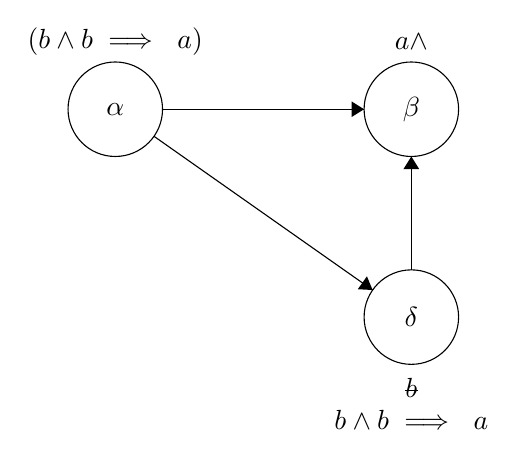
\begin{tikzpicture}[scale=0.2] 
\tikzstyle{every node}+=[inner sep=0pt] 
\draw [black] (21.9,-20.5) circle (3); 
\draw (21.9,-20.5) node {$\alpha$}; 
\draw [black] (40.7,-20.5) circle (3); 
\draw (40.7,-20.5) node {$\beta$}; 
\draw [black] (40.7,-33.7) circle (3); 
\draw (40.7,-33.7) node {$\delta$}; 
\draw (40.7,-16.2) node {$a\wedge\boa$}; 
\draw (40.7,-38.2) node {\sout{$\boxx{b}$}}; 
\draw (21.9,-16.2) node {$\boxx{(b\wedge\boxx{b}\implies\ a)}$}; 
\draw (40.7,-40.2) node {$b\wedge\boxx{b}\implies\ a$}; 
\draw [black] (24.9,-20.5) -- (37.7,-20.5); 
\fill [black] (37.7,-20.5) -- (36.9,-20) -- (36.9,-21); 
\draw [black] (24.36,-22.22) -- (38.24,-31.98); 
\fill [black] (38.24,-31.98) -- (37.88,-31.11) -- (37.3,-31.93); 
\draw [black] (40.7,-30.7) -- (40.7,-23.5); 
\fill [black] (40.7,-23.5) -- (40.2,-24.3) -- (41.2,-24.3); 
\end{tikzpicture} 
\end{center}

Ip) $\boxx{(a\wedge\boa\implies b)}\vee\boxx{(b\wedge\boxx b\implies a)}$

Ts) R debolmente connessa

Supponiamo per assurdo che R non sia debolmente connessa.

Consideriamo il caso in cui dallo stato $\alpha$ si raggiungano due
stati $\beta$ e $\gamma$, tali che $\nexists\delta:\,\beta R\delta\vee\gamma R\delta$.
Supponiamo inoltre che:

$\veraw{\mu}{\beta}{a\wedge\neg b}$

$\veraw{\mu}{\gamma}{b\wedge\neg a}$

avremo allora:

$\veraw{\mu}{\beta}{a\wedge\boa}$

$\veraw{\mu}{\gamma}{b\wedge\boxx b}$

ma, poichè l'antecedente è vero e il conseguente no, avremo anche:

$\nonveraw{\mu}{\beta}{a\wedge\boa}\implies b$

$\nonveraw{\mu}{\gamma}{b\wedge\boxx b}\implies a$

allora:

$\nonveraw{\mu}{\alpha}{\boxx{(a\wedge\boa\implies b)}\vee\boxx{(b\wedge\boxx b\implies a)}}$

che è assurdo, perchè va contro l'ipotesi. La tesi allora deve essere
valida.

\begin{center} 
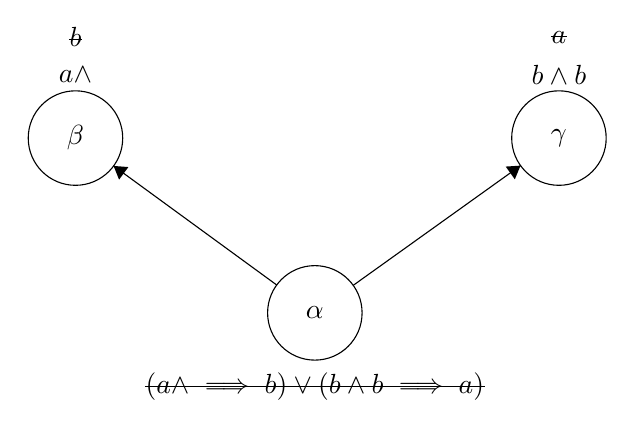
\begin{tikzpicture}[scale=0.2] 
\tikzstyle{every node}+=[inner sep=0pt] 
\draw [black] (42.2,-28.8) circle (3); 
\draw (42.2,-28.8) node {$\alpha$}; 
\draw [black] (27,-17.7) circle (3); 
\draw (27,-17.7) node {$\beta$}; 
\draw [black] (57.7,-17.7) circle (3); 
\draw (57.7,-17.7) node {$\gamma$}; 
\draw (27,-13.7) node {$a\wedge\boa$}; 
\draw (57.7,-13.7) node {$b\wedge\boxx{b}$}; 
\draw (27,-11.3) node {\sout{$b$}}; 
\draw (57.7,-11.3) node {\sout{$a$}}; 
\draw (42.2,-33.5) node {\sout{$\boxx{(a\wedge\boa\implies b)}\vee\boxx{(b\wedge\boxx b\implies a)}$}}; 
\draw [black] (44.64,-27.05) -- (55.26,-19.45); 
\fill [black] (55.26,-19.45) -- (54.32,-19.51) -- (54.9,-20.32); 
\draw [black] (39.78,-27.03) -- (29.42,-19.47); 
\fill [black] (29.42,-19.47) -- (29.77,-20.34) -- (30.36,-19.54); 
\end{tikzpicture} 
\end{center}



\chapter{Semantica}


\section{Formule equivalenti}

$a\equiv b$ cioè a è semanticamente equivalente a b, se:
\begin{itemize}
\item $\forall F\,\vera Fb\iff\vera Fa$
\item $\forall\mu\,\vera{\mu}b\iff\vera{\mu}a$
\item $\forall s\in S\,\veraw{\mu}sa\iff\veraw{\mu}sb$
\end{itemize}
si può anche dire che due formule sono semanticamente equivalenti
se:

$\vera ab\,\vee\,\vera ba$

Oppure infine se è valida in ogni frame:

$\valida{a\iff b}$


\section{Connettivi minimi}

Per ogni formula possiamo scriverne una equivalente che usa solo tre
connettivi: $\neg,\,\implies,\,\square$.

Infatti come è ben noto tutti i connettivi proposizionali si possono
esprimere in funzione della negazione e dell'implicazione, mentre
per quanto riguarda il connettivo diamond:

$\dia\equiv\neg\boxx{\neg a}$

Infatti:

se $\veraw{\mu}{\alpha}{\dia}$ allora

$\exists\beta:$$\alpha R\beta$ e $\veraw{\mu}{\beta}a$ da cui:

$\mu\nvDash_{\beta}\neg a$

per questo in $\alpha$ non vale $\boxx{\neg a}$ (perché non vale
$\neg a$ in $\beta$)

allora in $\alpha$ vale $\neg\boxx{\neg a}$ cioè $\veraw{\mu}{\alpha}{\neg\boxx{\neg a}}$
cioè la tesi. 

Similmente si dimostra l'altro verso dell'equivalenza.


\section{Logiche}


\subsection{Logica $\Lambda$}

Una logica $\Lambda$ su L è un insieme di fbf su L che: 
\begin{itemize}
\item contiene tutte le tautologie 
\item è chiusa rispetto al Modus Ponens 
\end{itemize}
Ad esempio; $PL(\phi)$ cioè i teoremi della logica proposizionale

Altro esempio $\Lambda_{C}=\{a\,|\,\vera F{a\: per}\ ogni\ F\in C\}$

infatti: 
\begin{itemize}
\item contiene tutte le tautologie perché sono vere mondo per mondo dappertutto 
\item MP : suppongo che in un mondo $\alpha$ accada che: $\nonveraw{\mu}{\alpha}b$
, $\veraw{\mu}{\alpha}a$ . Se vale anche $\veraw{\mu}{\alpha}{\implica ab}$
... l'antecedente è vero, quindi dato che l'implicazione è vera, deve
essere vero anche il conseguente da cui non può che essere $\veraw{\mu}{\alpha}b$ 
\end{itemize}
Una logica si dice \textbf{uniforme }se è chiusa rispetto a sostituzioni
uniformi cioè se sostituendo a una lettere uguali formule uguali in
una tautologia, ottengo una tautologia.

Es. $\Lambda_{C}=\{a\,|\,\vera F{a\: per}\ ogni\ F\in C\}$ NON è
uniforme infatti se considero $V(A)=S$, dove S sono tutti gli stati
possibili (mondi), vale anche $\veraw{\mu}{\alpha}A$, e cioè A è
una tautologia, se al posto di A sostituisco $B\wedge\neg B$ (falsa
in ogni modello e mondo) non ottengo una tautologia.


\subsection{Logiche modali normali}

Le logiche normali sono logiche che contengono lo schema K

$K:\,\boxx{(a\implies b)}\implies(\boa\implies\boxx b)$

Ed sono chiuse rispetto alla regola di necessitazione:

$RN:\,\dfrac{a}{\boa}$

La logica normale ha i seguenti assiomi:

$A1:\, a\implies(b\implies a)$

$A2:\,(a\implies(b\implies c))\implies((a\implies b)\implies(a\implies c))$

$A3:\,(\neg a\implies\neg b)\implies((\neg a\implies b)\implies a)$

$K:\,\boxx{(a\implies b)}\implies(\boa\implies\boxx b)$

$MP:\,\dfrac{a,\, a\implies b}{b}$

$RN:\,\dfrac{a}{\boa}$

L'intersezione di tutte le logiche normali, è una logica normale (ed
è la minima ) che non ha altri assiomi.

I teoremi sono le ultime formule della dimostrazione, ossia le formule
che ottengo dopo un numero finito di applicazione degli assiomi oppure
utilizzando la regola di necessiazione o il modus ponens.

La minima logica normale viene chiamata logica K.


\subsection{Teorema}

Sono equivalenti: 
\begin{enumerate}
\item $\Lambda$ è normale 
\item per ogni intero n $\geq0$,


$\teorema{a1\wedge a2\wedge...\wedge an}\implies a$ implica $\teorema{\boa1\wedge\boa2\wedge...\wedge\boa n}\implies\boa$

\item valgono:

\begin{enumerate}
\item $\teorema{\boxx T}$ 
\item $\teorema{\boa\wedge\boxx b}\implies\boxx{(a\wedge b)}$ 
\item $\teorema{\implica ab}$ implica $\teorema{\boa\implies\boxx b}$ 
\end{enumerate}
\end{enumerate}
Dimostrazione

$1\implies$2

per induzione.

se n = 0 allora $\teorema a$ allora $\teorema{\boa}$ per la regola
RN che vale in $\Lambda$ per ipotesi

se n > 0 (passo induttivo) suppongo valga l'antecedente, altrimenti
2 vale senz'altro;

si può dimostrare quindi nel seguente modo:

$\teolm{\Lambda}{a_{1}\wedge a_{2}\wedge...\wedge a_{n}n\implies a}$

$\teolm{\Lambda}{a_{1}\wedge a_{2}\wedge...\wedge a_{n-1}\implies(a_{n}\implies a)}$ 

$\teolm{\Lambda}{\boxx{a_{1}}\wedge\boxx{a_{2}}\wedge...\wedge\boxx{a_{n-1}}\implies\boxx{(a_{n}\implies a)}}$
-- per ipotesi di induzione

$\teolm{\Lambda}{\boxx{a_{1}}\wedge\boxx{a_{2}}\wedge...\wedge\boxx{a_{n-1}}\implies(\boxx{a_{n}\implies\boa}})$
-- per K

$\teolm{\Lambda}{\boxx{a_{1}}\wedge\boxx{a_{2}}\wedge...\wedge\boxx{a_{n-1}\wedge\boxx{a_{n}}}\implies\boa}$ 

E la tesi è dimostrata.

2$\implies$1

$\teolm{\Lambda}{(a\wedge(a\implies b))\implies b}$ -- per MP

$\teolm{\Lambda}{(\boa\wedge\boxx{(a\implies b))}}\implies\boxx b$
-- per enunciato 2

$\teolm{\Lambda}{\boxx{(a\implies b)}}\implies\boa\implies\boxx b$
-- che è K

Abbiamo ricavato usando solo il modus ponens e l'enunciato 2, l'assioma
K. segue quindi la tesi.

1$\implies3$

$\teolm{\Lambda}{\top}$

$\teolm{\Lambda}{\boxx{\top}}$-- per RN

$\teolm{\Lambda}{a\wedge b\implies a\wedge b}$ -- per tautologia
($a\implies a)$

$\teolm{\Lambda}{\boa\wedge\boxx b\implies}\boxx{(a\wedge b)}$ --
per proposizione 2

$\teolm{\Lambda}{a\implies b}$ -- per ipotesi

$\teolm{\Lambda}{\boxx{(a\implies b)}}$ -- per RN

$\teolm{\Lambda}{\boxx{(a\implies b)}\implies(\boa\implies\boxx{b)}}$
-- per K

$\teolm{\Lambda}{\boa\implies\boxx b}$ -- per MP

La tesi allora è verificata.

3$\implies$1

dimostriamo due tesi: che la 3 è chiusa rispetto alla necessitazione
e che implica l'assioma K.

$\teolm{\Lambda}a$

$\teolm{\Lambda}a\implies(\top\implies a)$ -- per A1

$\teolm{\Lambda}{\top\implies a}$ -- per MP

$\teolm{\Lambda}{\boxx{\top}\implies\boa}$ -- per 3.c

$\teolm{\Lambda}{\boa}$ -- per 3.a e MP

abbiamo così dimostrato la chiusura secondo la necessitazione.

$\teolm{\Lambda}{a\wedge b\implies c}$

$\teolm{\Lambda}{\boxx{(a\wedge b)\implies\boxx c}}$ -- per 3.c

$\teolm{\Lambda}{\boa}\wedge\boxx b\implies\boxx{(a\wedge b)}$ --
per 3.b

$\teolm{\Lambda}{\boa\wedge\boxx b\implies\boxx c}$ -- per la combinazione
delle due implicazioni precedenti

$\teolm{\Lambda}a\wedge(a\implies b)\implies b$ -- per tautologia

$\teolm{\Lambda}{\boa}\wedge\boxx{(a\implies b)}\implies\boxx b$
-- per applicazione dello schema $\boa\wedge\boxx b\implies\boxx c$
dimostrato precedentemente

$\teolm{\Lambda}{\boxx{(a\implies b)}\implies(\boa\implies\boxx{b)}}$

e così è dimostrato che K è implicato da 3. Il teorema dunque è dimostrato.


\section{Deducibilità di una formula}

Una formula a si dice deducibile da un insieme di formule $\Gamma$
in una logica $\Lambda$ e si scrive:

$\sintattica{\Gamma}{\Lambda}a$

se e solo se:

$\teorema{a_{1}\wedge\,...\,\wedge a_{n}\implies a}$

con $a_{1},\,...\,,\, a_{n}\in\Gamma$

Cioè, una formula a si dice deducibile da un insieme di formule $\Gamma$
se e solo se la congiunzione di formule che formano $\Gamma$ implica
la formula a

si noti che:

$\sintattica{\Gamma}{\Lambda}a\implies\sintattica{\{\boxx b\,|b\in\Gamma\}}{\Lambda}{\boa}$


\global\long\def\veraw#1#2#3{#1\models_{#2}#3}


\global\long\def\vera#1#2{#1\models#2}


\global\long\def\nonvera#1#2{#1\nvDash#2}


\global\long\def\nonveraw#1#2#3{#1\nvDash_{#2}#3}


\global\long\def\nonSem#1#2{#1\nvdash#2}


\global\long\def\nonSemW#1#2#3{#1\nvdash_{#2}#3}


\global\long\def\verita#1#2{#1\in V(#2)}


\global\long\def\entail#1#2{#1\models#2}


\global\long\def\semantica#1#2#3{#1\vdash_{#2}#3}


\global\long\def\semGen#1#2{#1\vdash#2}


\global\long\def\boxx#1{\square#1}


\global\long\def\diam#1{\diamond#1}


\global\long\def\dia{\diamond a}


\global\long\def\boa{\boxx a}


\global\long\def\noa{\sim}


\global\long\def\forhten#1#2#3{\forall#1#2\Rightarrow#3}


\global\long\def\implica#1#2{#1\Rightarrow#2}


\global\long\def\teorema#1{\vdash_{\Lambda}#1}


\global\long\def\teorGamma#1{\Gamma\vdash_{\Lambda}#1}


\global\long\def\teoa{\teorGamma a}


\global\long\def\consist{\mbox{\ensuremath{\Lambda}}-consistente}


\global\long\def\consMax{\Lambda-consistente\: massimale}



\chapter{Verso la decidibilità - Logica determinata}


\section{Insieme $\Lambda$ consistente e sue proprietà}

Sia $\Lambda$ una logica (cioè ha tutte le tautologie ed è chiusa
rispetto al Modus Ponens)

$\Gamma$ si dice $\Lambda$-consistente se: $\nonSemW{\Gamma}{\Lambda}{\bot}$,
dove $\bot=A\wedge\sim A$

$\Delta${ si dice $\Lambda$}-consistente massimale se per ogni fbf
$a${ $a\in\Delta$} oppure $\sim a\in\Delta$ $ $\\




\textbf{Proprietà:}
\begin{enumerate}
\item Se $\teoa$ e $\Gamma\subseteq\Delta$ allora $\Delta\teorema a$.
Ovvero se alcune premesse non mi servono posso comunque metterle per
dedurre una formula
\item Se $\teorGamma a$ e $\Lambda\subseteq\Lambda'$ allora $\Gamma\vdash_{\Lambda'}a$.
Ovvero quello che posso dedurre in una logica più scarna (es. PL)
lo posso dedurre anche in una più ricca che la contien (es. Modale)
\item se $a\in\Gamma$ allora $\teoa$ . \\
Infatti $\teorema{a\implies a}$ è un teorema dato che $a\implies a$
è una tautologia
\item $\{a|\teoa\}$ è la minima logica che contiene $\Gamma\cup\Lambda$.
Infatti posso dedurre tutte le tautologie da $\Gamma$, anche se non
userò nessuna formula di $\Gamma$ ma solo quelle che già sono nella
logica $\Lambda$
\item Se $\teoa$ e $\{a\}$$\teorema b$ allora $\teorGamma b$ \\
Infatti: per dedurre $a$ uso regole di inferenza, formule di $\Gamma$,
assiomi di $\Lambda$. Per arrivare in $b$ uso assiomi di $\Lambda$
e regole di inferenza, quindi posso arrivare da $\Gamma$ direttamente
in $b$ usando formule di $\Gamma$, regole di inf. e assiomi di $\Lambda$
\item Se $\teoa$ e $\teorGamma{\implica ab}$ allora $\teorGamma b$, dato
che $\Lambda$ è chiusa rispetto al MP
\item $\Gamma\cup\{a\}\teorema b$ se e solo se $\teorGamma{\implica ab}$
\\
\textbf{Andata}: $\teorema{a_{1}\wedge...\wedge a\wedge...\wedge}a_{n}\implies b$
(per definizione di teorema), si può portare $a$ alla destra dell'implicazione
$\teorema{a_{1}\wedge...\wedge}a_{n}\implies(a\implies b)$ \\
\textbf{Ritorno}: $\teorema{a_{1}\wedge}...\wedge a_{n}\implies(a\implies b)$,
basta portare $a$ tra le $ $and.
\item $\teoa$ se e solo se $\Gamma\cup\{\sim a\}$ non è $\Lambda$-consistente
\\
\\
\textbf{Andata}: $\teoa$, $\Gamma\teorema{\sim a}$, posso dedure
$\bot$ che è contro la definizione di $\Lambda$-consistenza\\
\textbf{Ritorno}: Se$ $$\Gamma\cup\{\sim a\}$ non è $\Lambda$-consistente,
allora $\Gamma\cup\{\sim a\}\teorema{\bot}$ da cui per 7. \\
$\Gamma\teorema{\sim a\implies\bot}$ (sposto $\sim a$ a destra e
metto l'implica), \\
Dato che $(\sim a\implies\bot)\implies a$ è una tatutologica, per
MP ottengo\\
$a$
\item $\Gamma$ è $ $$\consist$ se e solo se $\exists\beta:\nonSem{\Gamma}{_{\Lambda}\beta}$
\\
\textbf{Andata}: Basta prendere $\sim a\wedge a$\\
\textbf{Ritorno}: Se deducessi tutte le formule ($\sim$$\exists\beta:\nonSem{\Gamma}{_{\Lambda}\beta}$
significa $\forall\beta:\teorGamma{\beta}$) , potrei dedurre anche
$\bot$, da cui la non consistenza
\item $\Gamma$ è $\consist$ se per ogni $a$ \\
$\Gamma\cup\{a\}$ o $\Gamma\cup\{\sim a\}$ è $\consist$\\
se $\teoa$ allora $ $$\Gamma\cup\{\sim a\}$ non è consistente perché
con $a$ e $\sim a$ posso dedurre $\bot$, ma $\Gamma\cup\{a\}$
lo è \\
se $\Gamma\teorema{\sim a}$ allora $ $$\Gamma\cup\{\sim a\}$ è
consistente ma non $\Gamma\cup\{a\}$
\item $\bot$$\notin\Gamma$ se $\Gamma$ è $\consist$ (altrimenti potrei
dedurlo per il 3.)
\item Se $\Delta$è $\consist\: massimale$ e $\Delta\teorema a$ allora
$a\in\Delta$\\
se $a\notin\Delta$ allora $\sim a\in\Delta$ (dato che $\Delta$è
massimale) \\
ma se $\Delta$ contiene $\sim a$ allora per il 2.)\\
$\Delta\teorema{\sim a}$ , che insieme a $\Delta\teorema a$ mi da
$\Delta\teorema{\bot}$
\item Se $\Delta$ è $\consMax$ e $ $$a\in\Delta$. $\implica ab\in\Delta$
allora $b\in\Delta$. \\
Lo si vede subito usando 2.) se tutti e tre, e poi 6.) (deduco $a$,
$\implica ab$, allora deduco anche $b$)\end{enumerate}

 
\end{document}
